\chapter{Results}
\label{ch:results}

This chapter demonstrates side-by-side subfigures and a table that can break
across pages.

\section{Qualitative Results}
\label{sec:qualitative}

% Two images side by side with the subcaption package. Each subfigure
% gets its own caption and label; \ref produces e.g. "4.1a", and
% \subref produces just "a".
Figure~\ref{fig:results} shows two views of the same result.

\begin{figure}[h]
    \centering
    \begin{subfigure}[t]{0.45\textwidth}
        \centering
        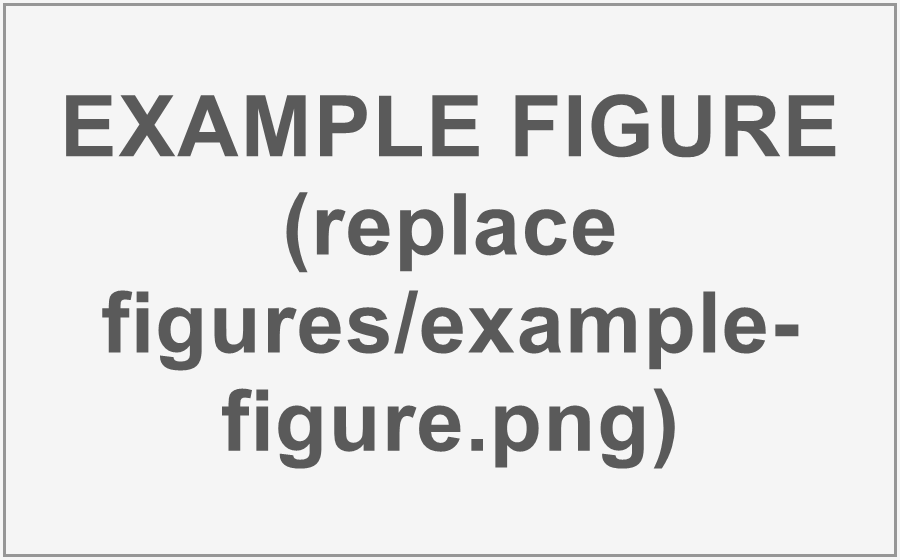
\includegraphics[width=\linewidth]{figures/example-figure.png}
        \caption{First view.}
        \label{fig:results-a}
    \end{subfigure}
    \hfill
    \begin{subfigure}[t]{0.45\textwidth}
        \centering
        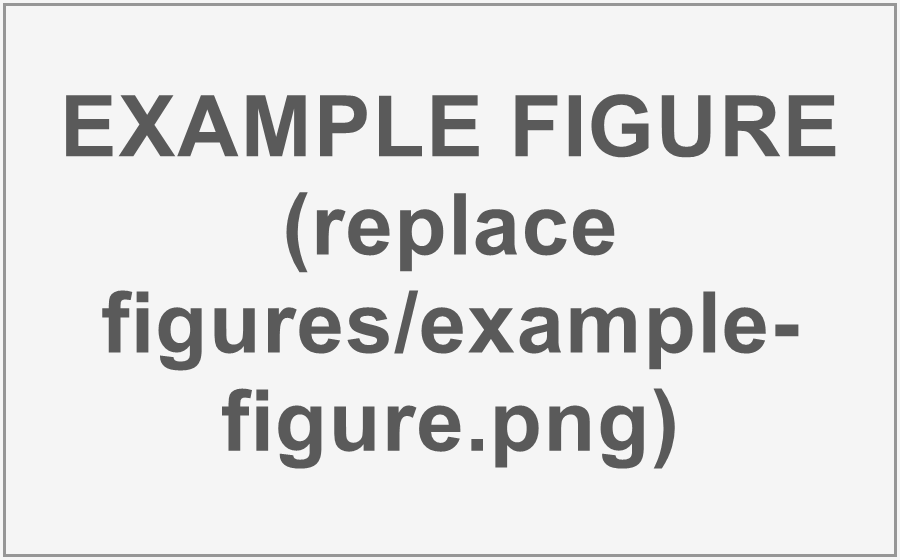
\includegraphics[width=\linewidth]{figures/example-figure.png}
        \caption{Second view.}
        \label{fig:results-b}
    \end{subfigure}
    \caption{A single figure made of two subfigures,
             \subref{fig:results-a} and \subref{fig:results-b}.}
    \label{fig:results}
\end{figure}

\section{Quantitative Results}
\label{sec:quantitative}

% A longtable automatically continues onto the next page and repeats the
% header row. Unlike a normal table it is NOT a float, so it goes exactly
% where you put it.
The full set of measurements is reported in Table~\ref{tab:long}.

\begin{longtable}{|c|c|c|}
    \caption{A long table that can break across pages.}
    \label{tab:long}\\
    \hline
    \textbf{Run} & \textbf{Accuracy} & \textbf{Time (s)} \\ \hline
    \endfirsthead
    \hline
    \textbf{Run} & \textbf{Accuracy} & \textbf{Time (s)} \\ \hline
    \endhead
    1 & 0.91 & 12.3 \\ \hline
    2 & 0.93 & 11.8 \\ \hline
    3 & 0.95 & 12.1 \\ \hline
\end{longtable}
